\documentclass[11pt,a4paper]{article}
\usepackage[margin=28mm]{geometry}
\usepackage[T1]{fontenc}
\usepackage{lmodern}
\usepackage{microtype}
\usepackage{amsmath,amssymb,amsthm}
\usepackage{mathtools}
\usepackage{tikz}
\usetikzlibrary{arrows.meta,positioning}
\usepackage[hidelinks]{hyperref}
\hypersetup{
  pdftitle={Brownian continuum random tree limits of finite Fortuin--Kasteleyn maps above four},
  pdfauthor={OpenAI},
  pdfsubject={Finite-volume graph-metric scaling of critical FK planar maps for q greater than four}
}
\setlength{\emergencystretch}{2em}
\numberwithin{equation}{section}
\newtheorem{theorem}{Theorem}[section]
\newtheorem{proposition}[theorem]{Proposition}
\newtheorem{lemma}[theorem]{Lemma}
\newtheorem{corollary}[theorem]{Corollary}
\theoremstyle{definition}
\newtheorem{definition}[theorem]{Definition}
\theoremstyle{remark}
\newtheorem{remark}[theorem]{Remark}
\renewcommand{\P}{\mathbb P}
\newcommand{\E}{\mathbb E}
\newcommand{\R}{\mathbb R}
\newcommand{\N}{\mathbb N}
\newcommand{\1}{\mathbf 1}
\newcommand{\dd}{\mathrm d}
\newcommand{\op}{o_{\P}}
\newcommand{\Op}{O_{\P}}
\newcommand{\GHP}{\mathrm{GHP}}

\title{Brownian continuum random tree limits of finite Fortuin--Kasteleyn maps above four}
\author{OpenAI}
\date{September 24, 2026}

\begin{document}
\maketitle

\begin{abstract}
We prove the finite-volume continuum-random-tree prediction for critical
Fortuin--Kasteleyn planar maps at every fixed $q>4$. After rescaling graph
distances by a constant times $n^{-1/2}$, an $n$-edge map with normalized
degree measure converges to the Brownian continuum random tree in the
Gromov--Hausdorff--Prokhorov topology. The convergence holds through all
positive integer sizes.
\end{abstract}

\section{Introduction}\label{sec:introduction}

A large planar map can contain many cycles while its distances, viewed
on a sufficiently large scale, approach those of a tree. We prove that
this happens for critical Fortuin--Kasteleyn maps at every fixed
$q>4$: their finite-volume metric scaling limit is the Brownian
continuum random tree.

Two features of this statement require separate work. The probability
law is conditioned on the size of the entire finite map, and the metric
uses all its edges. A limit of an unconditioned encoding walk does not
supply either conclusion. Our proof identifies an exact marked block
tree, proves that its offspring law is critical with finite variance,
and controls the graph distances contributed by its blocks uniformly
over all ancestral paths.

\subsection{The finite model and the main result}

A \emph{rooted planar map} is a connected graph embedded in an oriented
sphere, up to orientation-preserving homeomorphism, with a distinguished
oriented edge, or \emph{dart}. Loops and multiple edges are allowed.
For an edge subset $A\subseteq E(M)$, let $k_M(A)$ be the number of
components of the spanning graph $(V(M),A)$, counting isolated vertices.
For $q>4$ and $n\ge1$, sample a pair $(M_n,A_n)$ with $|E(M_n)|=n$
according to
\begin{equation}\label{eq:finite-law}
 \P\big((M_n,A_n)=(M,A)\big)
  =\frac{1}{Z_{n,q}}\,
    q^{\,k_M(A)+(|A|-|V(M)|)/2}.
\end{equation}
Equivalently, the weight is $q^{\ell(M,A)/2}$, where
$\ell(M,A)=2k_M(A)+|A|-|V(M)|$ is the number of FK interface loops.
Let $d_n$ be graph distance on $V(M_n)$ using every edge of $M_n$, and put
\begin{equation}\label{eq:degree-measure}
 \mu_n(\{v\})=\frac{\deg_{M_n}(v)}{2n}.
\end{equation}
A loop contributes two to the degree.

Let $e$ be a standard normalized Brownian excursion on $[0,1]$. For
$s,t\in[0,1]$, define
\[
 d_e(s,t)=e(s)+e(t)-
   2\min_{r\in[s\wedge t,s\vee t]}e(r).
\]
The quotient by $d_e=0$, equipped with its induced metric and the
pushforward $\mu_e$ of Lebesgue probability measure, is denoted
$(\mathcal T_e,d_e,\mu_e)$. We use this normalization throughout.

\begin{theorem}\label{thm:main}
For every fixed real $q>4$, there is a deterministic constant
$c(q)\in(0,\infty)$ such that, as $n\to\infty$ through all positive
integers,
\[
 \big(V(M_n),c(q)n^{-1/2}d_n,\mu_n\big)
 \ \Longrightarrow\ (\mathcal T_e,d_e,\mu_e)
\]
in the Gromov--Hausdorff--Prokhorov topology on compact metric probability
spaces modulo measure-preserving isometry.
\end{theorem}

The root and FK decoration are forgotten in this convergence.
We recall the correspondence estimate for this topology in
Section~\ref{metric:section}, where the metric and measure comparison is
completed.

\subsection{History and the ingredients of the proof}

The random-cluster representation of Fortuin and Kasteleyn connects
percolation and Potts-type spin systems through a weight on edge
subsets~\cite{FortuinKasteleyn1972}. On a random planar map, the map
itself is also sampled, so the cluster weight changes the underlying
geometry. Sheffield's inventory model encodes this joint randomness by
two types of burgers, two fixed order types, and flexible orders that
take the freshest available burger~\cite{Sheffield2016}. Its parameter
$p=\sqrt q/(\sqrt q+2)$ places $q>4$ exactly in the regime $p>1/2$.
Sheffield's unconditioned walk theorem identifies the transition at
$q=4$: above it, the limiting inventory fluctuations are
one-dimensional~\cite[Theorem~2.5]{Sheffield2016}.

The finite-volume CRT prediction appears in Sheffield's
appendix~\cite{Sheffield2016}. Feng restates it as
Conjecture~1.2 and proves an infinite-volume
counterpart~\cite{Feng2026}: his Theorem~1.3 concerns an infinite FK map
and convergence to an infinite continuum random tree in the
\emph{local} Gromov--Hausdorff--Prokhorov topology.
Theorem~\ref{thm:main} realizes the finite-volume prediction in the
compact topology, with the degree probability measure and all integer
edge sizes. It is proved directly under the finite law, not deduced
from the infinite-map limit.

The contrast with the other FK regimes is geometric. Companion results
for $0<q<4$ give Liouville quantum gravity sphere limits in the
metric-measure and conformal settings~\cite{SubcriticalMetric2026,SubcriticalConformal2026};
the critical companion treats the sphere and FK-map geometry at
$q=4$~\cite{CriticalFK2026}. Above four the limit here is instead a
tree. These companion results provide context and are not inputs to
the proof.

The finite-map encoding has a longer combinatorial ancestry. Mullin
enumerated tree-rooted maps~\cite{Mullin1967}, and Bernardi gave an
explicit bijective account using shuffles of two parenthesis
systems~\cite{Bernardi2007}. Bernardi's embedding activities and
subgraph correspondences relate these encodings to the Tutte
polynomial~\cite{Bernardi2008,Bernardi2008Subgraphs}; Sheffield combines
this structure with flexible orders to obtain the FK
weights~\cite[Section~4]{Sheffield2016}. We rederive the needed finite
identity with our dart-rooting and activity conventions in
Section~\ref{word:section}. The derivation fixes the exact conditioned
map law, including loops, links, and the trivial map used in the
generating function.

The inventory estimates below also build on specific earlier work.
Sheffield analyzes the first backward surviving burger and computes
the associated mean reduced length in
\cite[Section~3.1, Lemma~3.1]{Sheffield2016}. We use the same stationary
covariance and stopping method to prove the strict drift estimate
needed here. The reduced ladder excursions, balanced burger frequencies,
positive flexible-order frequency, and enclosing empty intervals of
\cite[Section~3.3]{Sheffield2016} are close predecessors of our cut
construction. We use these ideas to obtain the uniform matching
probability and generating-function lower bound needed for the
finite-map argument; both estimates are proved in
Section~\ref{ladder:section}.

The block decomposition itself goes back to
Tutte~\cite[Section~6]{Tutte1963}. Addario-Berry makes its exact
corner-indexed tree, including empty insertions and the $2n+1$ node
count, explicit for uniform maps~\cite[Section~2 and Proposition~3.1]{AddarioBerry2019}.
Stufler treats block-weighted maps in the general framework of enriched
trees and describes their metrics in terms of
corners~\cite[preprint Sections~6.1.5 and~6.8.3]{Stufler2020}.
Exponential tilting preserves a simply generated tree law conditional
on its size; Janson gives the associated offspring moment
formulas~\cite[Section~4]{Janson2012}.
The CRT limits for subcritical graph classes of Panagiotou, Stufler,
and Weller~\cite{PanagiotouStuflerWeller2016}, and the block-map results
in~\cite[preprint Theorems~6.60 and~6.62]{Stufler2020}, establish the principle
that graph distance is asymptotic to a constant times ancestral depth.
Their analytic hypotheses supply exponential moments. Our endpoint
argument establishes only finite offspring variance, so we retain a
path estimate that requires no exponential or third moment.

A recent result of Stufler~\cite[Theorem~1.2 and Lemma~9.1]{Stufler2026}
proves finite-variance degree-measure Gromov--Hausdorff--Prokhorov CRT
limits for maps whose block weights are functions of the block's edge
count. It also uses the exact corner-to-degree correspondence. In that
model blocks of a given size are uniform, and the metric argument uses
diameter estimates for uniform nonseparable maps. The FK weight of a
block instead depends on its shape, not only on its edge count. We must
prove finite variance for these weights and control their particular
metric marks.
The quadratic inverse criterion in Section~\ref{block:section} and the
finite-second-moment path argument in Section~\ref{tree:section}
provide those steps.

Finally, the limiting tree and the probabilistic tools have classical
origins. Aldous introduced the Brownian continuum random tree and its
finite-variance branching-process limit~\cite{Aldous1993}; Duquesne
developed the stable-domain extension~\cite{Duquesne2003}.
Marckert and Mokkadem proved joint depth-first process convergence to
the same excursion under stronger moment
hypotheses~\cite{MarckertMokkadem2003}. We use Broutin and Marckert's
joint coding theorem and conditioned-degree lemma in a formulation
that gives the height, contour, and walk limits jointly under a finite
second moment, through every attainable size~\cite{BroutinMarckert2014}.
The attainable tree sizes here are exactly the odd integers. The marked
ancestral-path calculation uses the size-biased spine method of
Lyons, Pemantle, and Peres~\cite[Section~2]{LyonsPemantlePeres1995}.
The truncation that makes it uniform over all nodes is proved below.


\subsection{Proof roadmap}

Section~\ref{word:section} expresses the total weight of $n$-edge maps,
up to an explicit exponential factor, as the probability that an
independent-letter inventory word of length $2n$ matches completely.
Ignoring burger types turns such a word into a nonnegative simple-walk
excursion. The resulting Catalan upper bound shows that the map
generating function is finite at the parameter selected by the word
law.

For a complementary lower bound, fix a boundary between two letters.
Scan to its left until the number of burgers minus orders first reaches
$h$, and to its right until that number first reaches $-h$.
Section~\ref{ladder:section} uses strict inventory drift and comparisons
of burger supply with order demand to prove that the whole interval
matches with probability bounded below uniformly in $h$.
Counting these intervals, together with a random-walk hitting-time
estimate, gives a square-root lower bound for the derivative of the map
series.

Section~\ref{block:section} decomposes a map into nonseparable pieces,
called blocks, joined at vertices. A corner is the sector between
successive incident darts; each block corner is an ordered attachment
slot, with an empty insertion recorded by a leaf. The exact substitution
equation for these attachments combines with the two word estimates to
force criticality and finite offspring variance, without analytic
continuation beyond the convergence endpoint. The resulting marked
Galton--Watson tree has exactly $2n+1$ nodes for an $n$-edge map.

Finally, Section~\ref{tree:section} combines the joint conditioned-tree
coding limit with uniform laws for the distance marks accumulated along
ancestral paths. Reversing the child order at every node gives a second
depth-first walk; the two walks control large marks using only the
second offspring moment. Section~\ref{metric:section} converts this path
estimate into a uniform comparison of map and tree distances. The
corners push uniform nonroot-node mass to the degree measure exactly,
which completes the metric probability-space comparison.

All constants may depend on the fixed parameter $q$. No uniform
statement as $q$ approaches $4$ is asserted.

\section{Words and strict drift}\label{word:section}

Fix $q>4$, and put
\begin{equation}\label{word:parameters}
 t=\sqrt q,\qquad p=\frac{t}{t+2},\qquad u=\frac{1-p}{16}.
\end{equation}
Thus $1/2<p<1$. For a rooted connected planar map $M$, define
\begin{equation}\label{word:weight}
 a(M)=\sum_{A\subseteq E(M)}
       t^{\,2k_M(A)+|A|-|V(M)|-1}.
\end{equation}
The decoration-summed weight in \eqref{eq:finite-law} is $t\,a(M)$. Since this
factor is independent of $M$, the marginal law of $M_n$ assigns
probability proportional to $a(M)$ among rooted maps with $n$ edges.
We also adjoin a trivial one-vertex, zero-edge map, whose weight is $1$,
and set
\[
 a_n=\sum_{\substack{M\text{ rooted planar map}\\ |E(M)|=n}}a(M),
 \qquad a_0=1.
\]
A directed root is a distinguished dart; in particular, a loop has two
darts. Rooted maps are counted up to root-preserving,
orientation-preserving isomorphism.

\subsection{Reduction of words}

Consider independent letters from the alphabet
\[
 \mathtt b_1,\ \mathtt b_2,\ \mathtt o_1,\ \mathtt o_2,\ \mathtt F
\]
with probabilities
\begin{equation}\label{word:letterlaw}
 \P(\mathtt b_1)=\P(\mathtt b_2)=\frac14,
 \qquad
 \P(\mathtt o_1)=\P(\mathtt o_2)=\frac{1-p}{4},
 \qquad \P(\mathtt F)=\frac p2.
\end{equation}
The letters $\mathtt b_i$ create burgers of type $i$. Read a word from
left to right. An order $\mathtt o_i$ removes the freshest remaining
burger of type $i$, and a flexible order $\mathtt F$ removes the freshest
remaining burger of either type. An order with no eligible burger is
unfilled; it is never served by a later burger.

The \emph{reduction} of a finite word is its list of unfilled orders,
followed by its list of surviving burgers, with each list retaining its
original chronology. A word is \emph{empty-reducing} if both lists are
empty. Throughout, a list of burgers is ordered from oldest to freshest.

\begin{lemma}[Reduction above an older supply]\label{word:reduction}
Feed a finite word an arbitrary older list of burgers. Every match
between two letters of the word is the same as when the word is read
from an empty supply. The orders unfilled in the latter evaluation act
on the older list in their original chronology, and the surviving burgers
of the word remain above the surviving older burgers. In particular,
finite words may be replaced by their reductions when concatenating
them. Once a suffix has a surviving burger, its freshest survivor is
unchanged by prepending further letters.
\end{lemma}

\begin{proof}
Call burgers created within the word new. At each order, an eligible new
burger is fresher than every old burger and therefore has priority.
Induction over the letters shows that the available new burgers evolve
exactly as they do with empty initial supply. Only orders for which no
eligible new burger exists can affect the old supply, and they do so in
their original order. The new survivors lie above all remaining old
burgers, which proves the first assertion and the concatenation rule.
To obtain the last assertion, first evaluate the prepended word and then
apply the rule to the original suffix. Its surviving burgers remain
unchanged and lie above any extra surviving supply.
\end{proof}

\subsection{An exact counting identity}

The tree-rooted-map encoding goes back to Mullin~\cite{Mullin1967};
Bernardi gives its two-parenthesis formulation~\cite{Bernardi2007}.
The inventory encoding with flexible orders is due to
Sheffield~\cite[Section~4]{Sheffield2016}.
We give the finite weighted identity in the form needed here. Its proof
uses a spanning-tree expansion determined by the embedding; related
embedding-based activity expansions of the Tutte polynomial were
introduced by Bernardi~\cite{Bernardi2008}. The activity convention below
is fixed explicitly, and the identity is proved directly.

\begin{proposition}[Finite word identity]\label{word:identity}
For every integer $n\ge0$, an independent word of length $2n$ satisfies
\begin{equation}\label{word:identity-equation}
 \P(\text{the word is empty-reducing})=a_nu^n.
\end{equation}
\end{proposition}

\begin{proof}
We give the bijection and the weight calculation, including their rooting
conventions.

\paragraph{Typed words and spanning trees.}
In an empty-reducing word, replace each flexible order by the fixed type
of the burger it consumes. The resulting \emph{identified word} has two
types of opening symbols, the burgers, and matching closing symbols,
the orders. Each type separately is a Dyck word: its running balance is
nonnegative, its final balance is zero, and matching follows its stack.
Thus an identified word is a shuffle of two Dyck words.

Such shuffles encode rooted planar maps with a distinguished spanning
tree $\mathcal T$. To see this, walk around a thickening of $\mathcal T$
in the orientation of the sphere, starting with the root dart. At a tree
dart, cross its edge and continue with the successor of the opposite dart
in its vertex's cyclic order. At a non-tree dart, continue with its
successor at the same vertex. This tour visits every dart exactly once.
The first and second occurrences of a tree edge give a type-1 opening
and closing; those of a non-tree edge give a type-2 opening and closing.
The tree pairs are noncrossing in contour order. The non-tree pairs are
also noncrossing, because their edges are disjoint arcs in the disk
complementary to the thickened tree.

Conversely, the type-1 symbols construct a plane tree by descending a new
edge at an opening and returning at its closing. Place the type-2 stubs
between successive tree steps in the given order, and join their matched
pairs in the complementary disk. Noncrossing matching determines these
arcs up to an orientation-preserving homeomorphism, so this constructs a
unique planar map. The first symbol specifies its root dart. The same
construction applies when there are no tree edges: all the stubs lie at
one vertex. At the end/start seam, retain the indicated cyclic order of
stubs. More explicitly, if $\alpha$ pairs matching positions and $\tau$
is the cyclic successor of positions, the reconstructed vertex successor
is $\tau\circ\alpha$ on tree darts and $\tau$ on non-tree darts.
This verifies that the two constructions are inverse, including the
rooting convention.

\paragraph{Flexible marks and activity.}
Say that two edges cross in the tour order when their occurrences
alternate. Such edges necessarily have opposite types. Call an edge
\emph{active} when it crosses no edge with a later first occurrence.
For an edge whose occurrences are $a<b$, its closing order can be made
flexible precisely when its burger is freshest among all burgers then
present. The obstruction is an edge with occurrences $c<d$ satisfying
$a<c<b<d$. Thus the eligible closings are exactly the active edges.
Any subset of them can be marked flexible while retaining all matches:
an induction through the word verifies that each changed order still
consumes the same burger. Conversely, every flexible mark in a word must
be eligible in its identified word.

Every fixed identified word with $n$ matched pairs has probability
$u^n$, since a burger and a fixed order contribute
$\frac14\frac{1-p}{4}=u$. Replacing a fixed order by a flexible one
multiplies its probability by
\[
 \frac{p/2}{(1-p)/4}=\frac{2p}{1-p}=t.
\]
If $b(M,\mathcal T)$ denotes the number of active edges, the total
probability of all its possible flexible markings is therefore
\begin{equation}\label{word:markedweight}
 u^n(1+t)^{b(M,\mathcal T)}.
\end{equation}

\paragraph{The activity sum.}
We next prove directly that
\begin{equation}\label{word:activity}
 a(M)=\sum_{\mathcal T\text{ spanning tree of }M}
          (1+t)^{b(M,\mathcal T)}.
\end{equation}
Evaluate the same expression on each connected residual map encountered
during edge deletion and contraction. Its weight does not require a
choice of root. Splitting its subset sum according to the
presence of an edge $e$ gives
\begin{equation}\label{word:deletion-contraction}
 a(M)=
 \begin{cases}
 a(M/e)+a(M\setminus e),&e\text{ is neither a bridge nor a loop},\\
 (1+t)a(M/e),&e\text{ is a bridge},\\
 (1+t)a(M\setminus e),&e\text{ is a loop}.
 \end{cases}
\end{equation}
For a nonloop present edge, contraction decreases $|A|$ and $|V|$ by
one and leaves the exponent unchanged. At a bridge, pairing the terms
with and without $e$ gives relative factors $1$ and $t$. At a loop,
including $e$ multiplies the corresponding deleted term by $t$.
The terminal one-vertex map has weight one.

Use the tour on the original darts to select the next edge in this
recursion. When an edge is first reached, a contraction declares it a
tree edge, and a deletion declares it a non-tree edge; thereafter use
the corresponding tour rule whenever that dart is visited. At a bridge
or loop the choice is forced. The next undecided edge depends only on
previous choices. Indeed, contracted edges form a forest, and deletion
of nonbridges preserves a connected residual graph, so every partial
branch has a spanning-tree completion. Its tour agrees with the partial
tour already traversed. Since a completed tree tour visits all darts,
the partial tour cannot close before every edge has been decided.
Consequently the recursion produces each spanning tree exactly once.

Fix a completed branch with spanning tree $\mathcal T$. A tree edge $e$
splits $\mathcal T$ into two components. A non-tree edge joins these two
components precisely when its occurrences alternate with those of $e$:
the contour interval cut out by the pair for $e$ visits exactly one side
of this tree cut. At the decision for $e$, earlier tree contractions
cannot identify the two sides, and the earlier non-tree edges have been
deleted. Hence $e$ is then a bridge if and only if no later non-tree
edge crosses its cut, which is exactly its activity condition.

Similarly, for a non-tree edge $e$, the tree edges crossing it in tour
order are exactly those on the tree path joining its endpoints. At its
decision, it has become a loop if and only if every edge of that path
has already been contracted. This again says exactly that no crossing
edge has a later first occurrence. The forced choices in the branch
are therefore its active edges. Equation~\eqref{word:deletion-contraction}
assigns that branch weight $(1+t)^{b(M,\mathcal T)}$, proving
Equation~\eqref{word:activity}.

There are no hidden symmetry factors in these counts. An automorphism
fixing the root dart and preserving the edge pairing and vertex cyclic
orders fixes every dart, by connectedness. Thus summing
Equation~\eqref{word:markedweight} over rooted map/tree pairs and using
Equation~\eqref{word:activity} proves
Equation~\eqref{word:identity-equation}. For $n=0$, both sides equal one.
\end{proof}

\begin{corollary}[Catalan upper bound]\label{word:catalan}
For every $n\ge0$,
\begin{equation}\label{word:catalan-equation}
 a_nu^n\le \frac{1}{4^n(n+1)}\binom{2n}{n}
          =O\bigl((n+1)^{-3/2}\bigr).
\end{equation}
\end{corollary}

\begin{proof}
Give a burger increment $+1$ and an order increment $-1$. By
Equation~\eqref{word:letterlaw}, these are independent symmetric
increments. An empty-reducing word must have a nonnegative running sum
and terminal sum zero: at every prefix, each order must already have
consumed a distinct preceding burger. Reflection gives exactly
$(n+1)^{-1}\binom{2n}{n}$ such sign sequences of length $2n$.
Apply Proposition~\ref{word:identity}, and then the usual central
binomial estimate.
\end{proof}

\subsection{The first backward survivor}

At a fixed boundary of an independent word, reveal letters backwards,
prepending one letter at each step. Write $S_j$ for the sum of the first
$j$ revealed burger-minus-order increments, with $S_0=0$. Let
\begin{equation}\label{word:J}
 J=\inf\{j\ge1:\text{the revealed suffix has a surviving burger}\}.
\end{equation}
At time $J$, the reduction consists of one burger and some number $K$
of fixed orders of the opposite type. To justify this assertion, note
that before the triggering letter the suffix has no surviving burgers.
That letter must therefore be a burger. By Lemma~\ref{word:reduction},
it survives precisely when none of the suffix's unfilled orders can
consume it; these orders must all be fixed orders of the other type.
In particular,
\begin{equation}\label{word:stopped-sum}
 S_J=1-K.
\end{equation}

This stopping variable is the one studied in Sheffield's inventory
analysis~\cite[Section~3.1]{Sheffield2016}.
His exact identity is $\E(1+K)=1/p$ in the present regime.
We prove the sufficient inequality $\E K\le1/(2p)<1$ directly,
retaining the covariance argument that makes the strictness visible.

\begin{proposition}[Strict drift]\label{word:drift}
The stopping time $J$ is almost surely finite, and
\begin{equation}\label{word:drift-equation}
 \E K\le\frac{1}{2p}<1.
\end{equation}
\end{proposition}

\begin{proof}
We first prove integrability, then exploit the type symmetry in a
stationary word to improve the bound.

\paragraph{A first integrability bound.}
If $S_j=1$, some burger must survive, so $J$ is no larger than the first
time the simple symmetric walk $S$ hits $1$. This hitting time is finite
almost surely. For example, stopping between $-r$ and $1$ gives
probability $r/(r+1)$ of reaching $1$ first, and letting $r$ increase
proves the assertion. Thus $J<\infty$ almost surely.

Stop the walk at the bounded time $J\wedge m$. Since its increments
have mean zero, Equation~\eqref{word:stopped-sum} gives
\begin{equation}\label{word:optional-stopping}
 \E[-S_m;J>m]=\E[1-K;J\le m].
\end{equation}
On $\{J>m\}$ there are no surviving burgers, so $S_m\le0$.
Consequently $\E[K;J\le m]\le\P(J\le m)$. Monotone convergence yields
$\E K\le1$. This uses no finite-mean assumption on $J$.

\paragraph{Typing flexible orders in a stationary word.}
Now take a two-sided independent sequence $(\omega_i)_{i\in\mathbb Z}$
with the letter law in Equation~\eqref{word:letterlaw}. At each boundary
immediately before index $i$, inspect the past until its first surviving
burger appears. The preceding argument and a countable intersection
make this possible almost surely for every $i$. By
Lemma~\ref{word:reduction}, the freshest survivor cannot change when
still older letters are prepended. Let $T_i\in\{+1,-1\}$ be its type
sign, with type 1 positive and type 2 negative.

Define the signed type increment $D_i$ by
\[
 D_i=
 \begin{cases}
 +1,&\omega_i=\mathtt b_1\text{ or }\mathtt o_2,\\
 -1,&\omega_i=\mathtt b_2\text{ or }\mathtt o_1,\\
 -T_i,&\omega_i=\mathtt F.
 \end{cases}
\]
This construction is shift-covariant, so $(D_i)$ is stationary. Each
$D_i$ is measurable with respect to raw letters at indices at most $i$.
Moreover, its flexible typing agrees with every flexible match internal
to any finite word: older supply cannot alter that match, by
Lemma~\ref{word:reduction}. Hence matched pairs cancel when signed
increments are summed.

Work at boundary $0$, and use $J,K$ for its backward variables. Set
\[
 T=T_0,\qquad D^{(m)}=\sum_{i=-m}^{-1}D_i.
\]
On $\{J=j\le m\}$ the final $j$ letters have signed sum $T(1+K)$:
the one burger and the $K$ opposite-type orders all contribute sign
$T$. The earlier signed sum $\sum_{i=-m}^{-j-1}D_i$ depends only on
raw letters earlier than $-j$. It is independent of the final $j$
letters, which determine $\{J=j\}$ and $T$ on that event.
Interchanging the two types preserves this event and reverses $T$,
so $\E[T\mathbf1_{\{J=j\}}]=0$. The earlier signed sum therefore
contributes zero in expectation against $T\mathbf1_{\{J=j\}}$.

On $\{J>m\}$ the reduced suffix consists only of orders. Internal
matched pairs cancel, so $|D^{(m)}|$ is at most the number of unfilled
orders, namely $-S_m$. Combining these observations with
Equation~\eqref{word:optional-stopping} gives
\begin{align}
 \E[T D^{(m)}]
 &\ge \E[1+K;J\le m]-\E[-S_m;J>m]\notag\\
 &=2\E[K;J\le m].\label{word:covariance}
\end{align}
Every variable in this calculation is integrable for fixed $m$; in
particular, $K\le m$ on $\{J\le m\}$.

\paragraph{Nonnegative second moments force strict drift.}
Let $V_m=\E[(D^{(m)})^2]$. Conditional on the raw past before index $0$,
the nonflexible letters have mean signed contribution zero, while the
flexible contribution has conditional mean $-(p/2)T$. Since $D_0^2=1$
and stationarity identifies the second moment of
$\sum_{i=-m}^{0}D_i$ with $V_{m+1}$, we obtain
\begin{equation}\label{word:variance-increment}
 V_{m+1}-V_m
   =1-p\E[T D^{(m)}]
   \le 1-2p\E[K;J\le m].
\end{equation}
If $2p\E K>1$, the last expression is bounded above by a strictly
negative constant for all sufficiently large $m$, by monotone
convergence. Summing Equation~\eqref{word:variance-increment} would then
force some $V_m$ to be negative. This contradiction proves
$\E K\le1/(2p)$, and $p>1/2$ makes the bound strictly smaller than one.
\end{proof}

\section{Ladder cuts and a coefficient lower bound}
\label{ladder:section}

Reduced excursions and balancing estimates for inventory words were
developed by Sheffield~\cite[Section~3.3]{Sheffield2016}.
We use these ideas to obtain a complete matching probability uniform in
the ladder height. Counting successfully matched intervals will then
give the coefficient estimate needed for finite-size conditioning.
The piece lengths need not have finite mean; the arguments below
integrate reduced lengths and use stationarity in the piece index.

Give each burger increment $+1$ and each order increment $-1$.
These increments form a simple symmetric random walk.
A left ladder piece, with law $L$, is obtained by sampling letters backwards
until their sum first reaches $+1$, then writing them in chronological order.
A right ladder piece, with law $R$, is obtained by sampling forwards until
the sum first reaches $-1$.
Both pieces are finite almost surely. Their net burger-minus-order counts
are respectively $+1$ and $-1$.

Fix a seam in a two-sided iid word. For $h\ge1$, take the letters on its
left up to the first backwards hit of $+h$, and the letters on its right
up to the first forwards hit of $-h$.
For each fixed $h$, the two resulting words are independent concatenations
of $h$ iid $L$-pieces and $h$ iid $R$-pieces.
Indeed, successive level-hitting times restart the iid sampling; reversing
the order of the $h$ left pieces preserves their joint iid law.
Our quantitative goal is the following bound on the finite-map weights.

\begin{proposition}[Coefficient lower bound]
\label{ladder:lower}
There is $c>0$ such that, for all real $x<1$ sufficiently close to $1$,
\begin{equation}
 \sum_{n\ge1} n a_n u^n x^n\ge c(1-x)^{-1/2}.
 \label{ladder:coefficient-bound}
\end{equation}
\end{proposition}

To prove this bound, we first show that the entire seam interval reduces
to the empty word with probability bounded below uniformly in $h$.
We construct boundaries that give burger-only reductions on the left
and orders-only reductions on the right, then compare their type counts.

\subsection{Stationary cuts}

We index pieces by $\mathbb Z$, with boundary $i$ immediately before piece $i$.
Thus the word between boundaries $a<b$ is the concatenation of pieces
$a,\ldots,b-1$.
We first record the averaging fact needed for observations that can depend
on infinitely many pieces.

\begin{lemma}[Stationary averaging]
\label{ladder:averaging}
Let $(Z_i)_{i\in\mathbb Z}$ be iid, and let $Y_i$ be the translates of an
integrable measurable function of the entire sequence $(Z_i)_{i\in\mathbb Z}$.
Then the averages of $Y_i$ in each index direction converge almost surely
to $\E Y_0$.
In particular, a shift-covariant set of boundaries having positive
probability at boundary $0$ has positive limiting density in both
directions. If $0$ belongs to this set, the last such boundary before $k$
is $k-o(k)$, and the first one after $-k$ is $-k+o(k)$.
\end{lemma}

\begin{proof}
An integrable function of a product sequence can be approximated in $L^1$
by bounded functions of finitely many coordinates.
The translates of a bounded finite-window function split into finitely
many iid subsequences. Their averages converge almost surely: for bounded
centered iid variables, the fourth moment of a partial sum of length $r$
is $O(r^2)$, so the deviation probabilities for their averages are summable.

For completeness, the approximation errors are controlled by the following
maximal inequality for any stationary nonnegative sequence $(U_i)$:
\begin{equation}
 \P\left(\sup_{r\ge1}\frac1r\sum_{i=1}^r U_i>\eta\right)
 \le \frac{\E U_0}{\eta},\qquad \eta>0.
 \label{ladder:maximal}
\end{equation}
To prove it, first allow witnessing intervals of length at most $s$.
Among violating starts in $1,\ldots,m$, select an interval at the first
such start, skip the starts it covers, and repeat.
The selected intervals are disjoint, cover every violating start, and lie
in $1,\ldots,m+s$.
Their sum exceeds $\eta$ times their total length, which is at least the
number of violating starts.
Taking expectations, dividing by $m$, and then letting $m$ and $s$ tend to
infinity proves Equation~\eqref{ladder:maximal}.
Apply this inequality to the absolute errors of the finite-window
approximations. As their $L^1$ errors tend to zero, the almost-sure
convergence of the averages follows. Reversing the indices proves the
other direction.

Apply the result to the indicator of the boundary set.
If $b_k\le k$ is its last boundary before $k$ and $d>0$ is its density,
the absence of boundaries between $b_k$ and $k$ gives
$d(k-b_k)=o(k)+o(b_k)=o(k)$.
The negative-index assertion is identical.
\end{proof}

\begin{definition}
For a two-sided iid sequence of $L$-pieces, a boundary $a$ is an
\emph{$L$-cut} if, for every $b>a$, the word between $a$ and $b$ has no
unfilled orders when evaluated from an empty supply.
For a two-sided iid sequence of $R$-pieces, a boundary $b$ is an
\emph{$R$-cut} if, for every $a<b$, the word between $a$ and $b$ leaves
no surviving burgers.
\end{definition}

\begin{lemma}[Positive probability of cuts]
\label{ladder:cuts}
Each fixed boundary has positive probability of being an $L$-cut and
positive probability of being an $R$-cut, in the respective piece laws.
Consequently both cut sets have positive limiting densities in both
index directions.
\end{lemma}

\begin{proof}
We use the strict drift estimate differently for the two cut probabilities.

\paragraph{Shortening left pieces.}
Recall the backwards stopping time $J$ and the integer $K$ from
Proposition~\ref{word:drift}.
At time $J$, the reduced word consists of one burger and $K$ fixed orders
of the opposite type, and $\E K<1$.
Parse backwards from the end of an $L$-piece using successive independent
copies of this stopping rule.
Before the end of any parsing step its relative sum is nonpositive:
a positive sum would force a surviving burger and hence an earlier stop.
The first hit of $+1$ therefore occurs at a parsing-step endpoint.
The number $N_L$ of steps is the first hit of $1$ by a walk whose iid
increments have law $1-K$.
Writing $\mu=1-\E K>0$, bounded stopping gives
\[
 \mu\,\E(N_L\wedge m)
   =\E\left[\sum_{j=1}^{N_L\wedge m}(1-K_j)\right]\le1.
\]
The bound holds because the increments are at most $1$ and the walk is
stopped on its first hit of $1$.
Thus $\E N_L\le1/\mu<\infty$.

Replace each parsing step by its reduction and put these reductions back
in chronological order.
Lemma~\ref{word:reduction} allows this replacement inside any larger word,
including with an older supply of burgers.
The resulting shortened $L$-piece has only burgers and fixed orders,
and its length $\ell$ satisfies
\begin{equation}
 \E\ell
 =\E\left[\sum_{j=1}^{N_L}(1+K_j)\right]
 =\E N_L\,\E(1+K)<\infty.
 \label{ladder:short-length}
\end{equation}
Here reaching parsing step $j$ depends only on the preceding steps, which
justifies the second equality.
The two net type counts in a shortened piece are integrable, sum to $1$,
and have the same law under exchange of the types.
Each therefore has expectation $1/2$.

Across successive forward $L$-pieces, the net count of each type has
positive drift.
Within a shortened piece, the deviation from its initial count is at most
its length. Moreover, for iid lengths of finite mean, $\ell_i/i\to0$
almost surely, by the integrable-tail bound and Borel--Cantelli.
The running infimum of each type count over all shortened letters is
therefore finite almost surely.
A sufficiently large deterministic starting supply of both types
prevents any unfilled order forever with positive probability.
A finite prefix of prescribed single-burger $L$-pieces creates this supply
with positive probability, independently of the remaining tail.
Starting with that prefix and an empty supply proves positive probability
of an $L$-cut at boundary $0$.
Only the shortened length in Equation~\eqref{ladder:short-length} was
integrated; no moment of the original ladder-piece length is needed.

\paragraph{Reversing right pieces.}
For an $R$-cut, we will show that a backward scan from a piece endpoint
has positive probability of never revealing a surviving burger.
Scan the letters backwards from boundary $0$ in a two-sided iid
$R$-piece sequence. Let $S_j$ be the burger-minus-order sum of the first
$j$ scanned letters. This scan has a different law from ordinary iid
backwards sampling.
The density of its first $m$ letters relative to ordinary iid backwards
sampling is
\begin{equation}
 2(-S_m)\,\1_{\{S_j<0\text{ for }1\le j\le m\}}.
 \label{ladder:reverse-density}
\end{equation}
To see this, use the last $h$ pieces for any $h>m$.
Their concatenation is an iid word stopped at its first hit of $-h$.
Write $W$ for its forward walk, started at $0$, and $\tau$ for this
hitting time. The reversed sums satisfy
\[
 S_j=W_\tau-W_{\tau-j}=-h-W_{\tau-j},\qquad 1\le j\le m.
\]
Since $W$ stays above $-h$ before $\tau$, a possible final string read
backwards has strictly negative partial sums.
If its total is $-r$, its chronological start is at
$-h+r$, where $1\le r\le m<h$.
Before killing at $-h$, the expected number of visits to this level is
$2r$: the walk visits it almost surely, and at each departure the
probability of being killed before returning is $1/(2r)$.
This last probability is one half times the elementary probability
$1/r$ of hitting the lower endpoint before returning from its adjacent
site; a departure upwards returns almost surely.
Each visit followed by the specified admissible string ends exactly at
the killing time. Summing over visits and multiplying by the iid
probability of that string proves Equation~\eqref{ladder:reverse-density}.

\paragraph{Removing the terminal order.}
The first backwards letter is necessarily an order.
After removing it, and restarting the sums at $0$, the remaining scan
has finite-dimensional density
\begin{equation}
 (1-S_j)\,\1_{\{\max_{1\le i\le j}S_i\le0\}}
 \label{ladder:remainder-density}
\end{equation}
relative to iid backwards sampling.
Indeed, the first order contributes $-1$; factoring its conditional order
law out of Equation~\eqref{ladder:reverse-density} leaves exactly
Equation~\eqref{ladder:remainder-density}. Explicitly, the original
probability of a specified order is $\tfrac12$ times its conditional
order probability; the $\tfrac12$ cancels the factor $2$ in the density.
The remaining density has no dependence on the removed order's type.

Apply the stopping rule $J$ to this remaining scan.
Under ordinary sampling, on $\{J=j\}$ the previous sums are nonpositive
and $S_j=1-K$.
The density in Equation~\eqref{ladder:remainder-density} on this event is
$K$: when $K=0$ the sign restriction fails and the density is zero;
when $K\ge1$ it is $1-S_j=K$.
Summing over the disjoint events $\{J=j\}$ shows that the probability,
under the remaining-scan law, of ever revealing a surviving burger is
$\E K$. This is a sum of finite-cylinder identities over disjoint
finite values of $J$, so countable additivity suffices; no optional
stopping of an unbounded density process or finite mean of $J$ is used.
With positive probability $1-\E K$, every finite scanned word instead
leaves no burgers. Appending the removed terminal order cannot create a
burger. In particular, every whole-piece word ending at boundary $0$
leaves no burgers, so this event implies an $R$-cut there.

Finally the cut indicators are shift-covariant functions of iid piece
sequences. Their positive densities follow from
Lemma~\ref{ladder:averaging}.
\end{proof}

\subsection{Stationary outputs and matching}

Between consecutive $L$-cuts $a<b$, the reduction is a burger-only word
of length $b-a$, since each piece has net count $+1$.
Assign these burgers in chronological order to the slots
$a,\ldots,b-1$.
The cut set is unbounded in both directions almost surely, so this
defines a stationary sequence of single burgers on all slots.
Similarly, between consecutive $R$-cuts $a<b$, assign the orders-only
reduction of length $b-a$ to these slots in chronological order.
Both output sequences are measurable shift-covariant functions of their
respective iid piece sequences; the cuts need not be independent.

The matching criterion below identifies the counts we must control:
the oldest available burgers and the orders that must still be filled
at the end.

\begin{lemma}[Bottom supply and terminal demand]
\label{ladder:matching}
Let a burger stack and an order word both have length $h$.
Suppose that, for every $1\le k\le h$ and each type $a$, the number of
fixed type-$a$ orders among the terminal $k$ orders is at most the number
of type-$a$ burgers among the original bottom $k$ burgers.
Then the greedy inventory rule matches all orders and leaves no burgers.
\end{lemma}

\begin{proof}
Suppose a first failure occurs, necessarily at a fixed order of some
type $a$: before a first failure there is one burger per remaining order,
so a flexible order can always be filled.
If no earlier flexible order consumed type $a$, all earlier consumption
of that type was fixed. The hypothesis at $k=h$ then rules out failure.

Otherwise consider the last earlier flexible consumption of type $a$.
Let it remove the burger at position $j$ in the original stack, counting
from the bottom, and let $k$ be the number of burgers immediately after
this removal.
While that burger was present, no fixed type-$a$ order could remove an
older type-$a$ burger, and no flexible order could remove anything older
than it. Hence every original type-$a$ burger below position $j$ is
still present just after this removal.
Because a flexible order takes the freshest burger overall, every
remaining burger is below position $j$; in particular $k\le j-1$.
The remaining type-$a$ supply is therefore at least its count in the
original bottom $k$ burgers.
By hypothesis this suffices for all fixed type-$a$ orders in the remaining
suffix of length $k$.
Until the alleged failure, no further flexible order consumes type $a$,
by our choice of the last such consumption. A failure is impossible.
\end{proof}

We now obtain uniform estimates for these supply and demand counts
from the stationary outputs.

\begin{lemma}[Output frequencies]
\label{ladder:frequencies}
Almost surely, each burger type has frequency $1/2$ in the stationary
$L$-output.
The stationary $R$-output has almost-sure frequencies
$(1-\rho)/2,(1-\rho)/2,\rho$ for the two fixed types and the flexible
orders, respectively, for a deterministic $\rho>0$.

On the event that $0$ is an $L$-cut, let $B_a(h,k)$ count type-$a$ burgers
among the bottom $k$ burgers of the reduction of the $h$ pieces starting
at $0$, where $1\le k\le h$.
Then, almost surely on this event,
\begin{equation}
 \lim_{k\to\infty}\sup_{h\ge k}
 \left|\frac{B_a(h,k)}k-\frac12\right|=0,
 \qquad a=1,2.
 \label{ladder:left-counts}
\end{equation}
On the event that $0$ is an $R$-cut, let $C_a(h,k)$ count fixed orders of
type $a$ among the terminal $k$ residual orders of the $h$ pieces ending
at $0$.
Then, almost surely on this event,
\begin{equation}
 \lim_{k\to\infty}\sup_{h\ge k}
 \left|\frac{C_a(h,k)}k-\frac{1-\rho}{2}\right|=0,
 \qquad a=1,2.
 \label{ladder:right-counts}
\end{equation}
\end{lemma}

\begin{proof}
Type exchange symmetry and Lemma~\ref{ladder:averaging} give the claimed
$L$-frequencies.
The event of an $R$-cut at $0$ depends only on pieces before $0$.
Independently requiring piece $0$ to be the single letter $F$, an event
of probability $p/2>0$, makes boundary $1$ a cut as well and places an
$F$ in output slot $0$.
Consequently
\[
 \rho\ge\P(0\text{ is an }R\text{-cut})\frac p2>0.
\]
Stationary averaging and type exchange symmetry give the remaining
$R$-frequencies.

For Equation~\eqref{ladder:left-counts}, let $b_k$ be the last $L$-cut
at or before $k$, on the event that $0$ is a cut.
It satisfies $k-b_k=o(k)$.
For every $h\ge k$, the bottom $b_k$ surviving burgers are exactly the
stationary output in slots $0,\ldots,b_k-1$:
the pieces after the cut $b_k$ require no older supply and cannot remove
these burgers, by Lemma~\ref{word:reduction}.
Thus the bottom-$k$ count differs from the corresponding stationary
prefix count by at most $k-b_k$, uniformly in $h$.
This proves Equation~\eqref{ladder:left-counts}.

For Equation~\eqref{ladder:right-counts}, take the first $R$-cut $c_k$
at or after $-k$; then $c_k=-k+o(k)$.
For every $h\ge k$, the whole-piece word from $-h$ to $c_k$ leaves no
burgers, by the definition of the cut at $c_k$.
Its residual orders cannot be served by later burgers and do not alter
the reduction of the suffix from $c_k$ to $0$.
The terminal $-c_k$ orders therefore agree exactly with stationary output
in these slots.
The possible discrepancy among the terminal $k$ orders is at most
$k+c_k=o(k)$, independently of $h$.
This proves Equation~\eqref{ladder:right-counts}.
\end{proof}

\subsection{Matching at a seam}

\begin{proposition}[Uniform success at a seam]
\label{ladder:uniform}
There is $\delta>0$, depending only on $p$, such that for every integer
$h\ge1$ the seam interval formed by the backwards hit of $+h$ and the
forwards hit of $-h$ reduces to the empty word with probability at least
$\delta$.
\end{proposition}

\begin{proof}
Choose
\[
 \frac{1-\rho}{2}<\alpha<\frac12.
\]
By Lemmas~\ref{ladder:cuts} and~\ref{ladder:frequencies}, for a sufficiently
large deterministic integer $B$, each of the following events has positive
probability in its respective stationary piece sequence:
\begin{align*}
 \mathcal G_L={}&\{0\text{ is an }L\text{-cut, and }
 B_a(h,k)\ge\alpha k
 \text{ for }a=1,2\text{ and all }h\ge k\ge B\},\\
 \mathcal G_R={}&\{0\text{ is an }R\text{-cut, and }
 C_a(h,k)\le\alpha k
 \text{ for }a=1,2\text{ and all }h\ge k\ge B\}.
\end{align*}
Indeed, increasing $B$ makes each event exhaust its positive-probability
cut event, up to a null set.
Take an integer $D\ge B$ with $\alpha D\ge B$.
The event $\mathcal G_R$ is measurable with respect to the past pieces,
so requiring the next $D$ pieces, indexed $0,\ldots,D-1$, to be single
flexible orders preserves positive probability.

Use independent stationary $L$- and $R$-sequences.
For the left word take $h$ pieces starting at $0$, and for the right word
take $h$ pieces ending at $D$.
Unconditionally these have exactly the independent ladder-piece laws
of the seam interval for each fixed $h$.
The event consisting of $\mathcal G_L$, $\mathcal G_R$, and the prescribed
$D$ flexible pieces has probability
\[
 \delta=\P(\mathcal G_L)\P(\mathcal G_R)(p/2)^D>0,
\]
independent of $h$.

On this event the left word reduces to $h$ burgers.
The right word reduces to $h$ orders: it is all flexible if $h\le D$;
otherwise it is the orders-only reduction of $h-D$ pieces ending at $0$,
followed by $D$ flexible orders.
Consider its terminal $k$ orders, with $k\le h$.
If $k\le D$, their fixed-type counts vanish.
If $k>D$ and $k-D\ge B$, each fixed-type count is at most
$\alpha(k-D)\le\alpha k$ by $\mathcal G_R$.
If $0<k-D<B$, each count is at most $B\le\alpha D\le\alpha k$.
In the last two cases $k\ge B$, so $\mathcal G_L$ supplies at least
$\alpha k$ burgers of each type in the bottom $k$ positions.
Thus every inequality in Lemma~\ref{ladder:matching} holds, including
the small values of $k$, and the interval reduces to the empty word.
\end{proof}

\subsection{Counting intervals through a seam}

\begin{proof}[Proof of Proposition~\ref{ladder:lower}]
Let $I_h$ be the seam interval in Proposition~\ref{ladder:uniform}.
Reflection for the simple symmetric walk bounds the hitting time of a
level $h$ by
\[
 \P(\tau_h>m)\le C_0\frac{h+1}{\sqrt m}.
\]
Consequently the two hitting lengths defining $I_h$, divided by $h^2$,
are tight uniformly over $h\ge1$.
Choose a deterministic $A<\infty$ large enough that
\[
 \P\bigl(I_h\text{ reduces to the empty word and }|I_h|\le Ah^2\bigr)
 \ge\delta/2,\qquad h\ge1.
\]
This follows by subtracting the length-tail probabilities from the success
probability; no independence between length and success is needed.
The intervals $I_h$ are distinct as $h$ varies, since the first-hitting
endpoints move strictly with the level.

There are exactly $2n-1$ deterministic intervals of length $2n$ using
letters on both sides of the seam.
Every empty-reducing word has even length.
By Proposition~\ref{word:identity} and Tonelli's theorem, the expected sum
of $x^{|I|/2}$ over all empty-reducing finite intervals through the seam is
\[
 \sum_{n\ge1}(2n-1)a_nu^n x^n.
\]
For $H=\lfloor(1-x)^{-1/2}\rfloor$, the distinct intervals
$I_1,\ldots,I_H$ therefore give
\begin{align*}
 \sum_{n\ge1}(2n-1)a_nu^n x^n
 &\ge \frac\delta2\sum_{h=1}^H x^{Ah^2/2}\\
 &\ge \frac\delta2 H\,x^{A/(2(1-x))}.
\end{align*}
The last factor is bounded away from zero as $x\uparrow1$, while
$H\asymp(1-x)^{-1/2}$.
Since $2n-1\le2n$, this proves
Equation~\eqref{ladder:coefficient-bound}.
\end{proof}

\section{The critical block tree}\label{block:section}

We now pass from the word estimates to an exact representation of the
finite map law. A \emph{corner} of a nonempty map is a sector between
successive darts at a vertex. Thus a map with $m$ edges has $2m$
corners, including two at a vertex carrying a single loop.

\subsection{Decomposition at corners}

The decomposition of a rooted map into a root block and corner insertions
goes back to Tutte~\cite[Section~6]{Tutte1963}. Addario-Berry makes its
even-offspring tree representation explicit for uniform
maps~\cite[Section~2 and Proposition~3.1]{AddarioBerry2019}; the
block-weighted form belongs to Stufler's enriched-tree
framework~\cite[preprint Section~6.1.5]{Stufler2020}.
We prove the rooted version here to keep the one-link and one-loop
conventions, trivial inserts, and exact finite weights explicit.

Our nontrivial \emph{blocks} are the rooted one-loop map and the rooted
nonempty connected loopless maps with at least two vertices and no
separating vertex. The one-link map is included: deleting either of its
vertices leaves a single vertex. Write $b_m$ for the total weight
$a(B)$ of the blocks with $m$ edges. In particular,
\begin{equation}\label{block:one-edge}
 b_1=2(1+t)>0.
\end{equation}

\begin{lemma}[Rooted corner substitution]\label{block:decomposition}
Every nontrivial rooted planar map is uniquely obtained from a rooted
block by inserting a rooted map, possibly trivial, in each of its
corners. A nonempty insert is attached at the origin of its root dart.
Moreover, $a$ is multiplicative when two maps are joined at one vertex.
Consequently, with
\[
 T(z)=\sum_{n\ge0}a_nz^n,\qquad
 \Phi(y)=1+\sum_{m\ge1}b_my^m,
\]
there is an identity of formal power series
\begin{equation}\label{block:equation}
 T(z)=\Phi\big(zT(z)^2\big).
\end{equation}
\end{lemma}

\begin{proof}
Suppose first that the root is not a loop. Take the maximal loopless
block containing the root edge. It is unique: the union of two
connected subgraphs without a separating vertex that share an edge
again has no separating vertex. An exterior path joining two different
vertices of this block, with interior disjoint from it, could be added
without producing a separating vertex. Thus every component outside the
block attaches at one block vertex.

Each face boundary of a loopless block visits a given vertex at most
once. Indeed, if two distinct sectors at a vertex belonged to the same
face, a simple curve through that face joining the sectors and closed
at the vertex would separate incident edges on its two sides.
Connectivity after deleting the vertex rules this out. The assertion
also holds for a one-link block. Planarity therefore places each
outside component in a unique corner of its attachment vertex.
Extra loops at a block vertex lie in such corners as well. Group all
parts in each corner into one insert.

If the root is a loop, take that loop as the root block. Its two sides
are its two corners, and the parts on either side form the two inserts.
In both cases a nonempty insert is rooted at the first outgoing dart
in its corner sector, in the oriented cyclic order. Conversely, glue
an arbitrary rooted insert at each corner, identifying its root origin
with the corner vertex and starting its cyclic order with its root dart.
This reconstructs the map and its rotations uniquely. Each insertion
meets the root block at only one vertex, so it cannot enlarge that
block. These constructions are inverse.

Rooting also identifies the corners individually. Indeed, an
automorphism fixing a root dart and preserving vertex rotations and
edge reversal fixes all darts by connectedness. We may thus choose a
deterministic order of the $2m$ corners of every rooted block, with no
symmetry divisor.

For the weight claim, join $M_1$ and $M_2$ at one vertex and write an
edge subset as $A_1\cup A_2$. The number of components and the number
of vertices are, respectively,
\[
 k_{M_1}(A_1)+k_{M_2}(A_2)-1,\qquad
 |V(M_1)|+|V(M_2)|-1.
\]
The exponent $2k+|A|-|V|-1$ is therefore the sum of the two exponents.
Summing independently over $A_1,A_2$ proves multiplicativity.
A size-$m$ root block contributes $b_mz^mT(z)^{2m}$; adding the
trivial map gives \eqref{block:equation}.
\end{proof}

\subsection{An endpoint criterion for finite variance}

An $m$-edge block supplies $2m$ child slots, so the first two offspring
moments will be controlled by the first two derivatives of the block
series. The next lemma extracts the required endpoint identities and
bounds from the word coefficient estimate.

\begin{lemma}[Quadratic inverse criterion]\label{block:critical}
Suppose $T$ and $\Phi$ have nonnegative coefficients and constant
term $1$, and satisfy \eqref{block:equation}. Let $u>0$ satisfy
$T(u)<\infty$, and suppose that, for some $c>0$,
\begin{equation}\label{block:lower-assumption}
 \sum_{n\ge1}na_nu^nx^n\ge c(1-x)^{-1/2}
 \qquad\text{for all $x<1$ sufficiently close to $1$}.
\end{equation}
Put $\tau=T(u)$ and $v=u\tau^2$. Then
\begin{equation}\label{block:critical-equations}
 \Phi(v)=\tau,\qquad
 2v\Phi'(v)=\Phi(v),\qquad
 \Phi''(v)<\infty,
\end{equation}
where endpoint derivatives denote the corresponding nonnegative series.
\end{lemma}

\begin{proof}
Integrating \eqref{block:lower-assumption} gives, for $z<u$ close to $u$,
\begin{equation}\label{block:square-root-gap}
 \tau-T(z)
 =\int_{z/u}^{1}\frac1x
        \sum_{n\ge1}na_nu^nx^n\,\dd x
 \ge c_1\sqrt{u-z}.
\end{equation}
All integrands are nonnegative, so monotone convergence justifies the
endpoint integration. The map
\[
 y(z)=zT(z)^2
\]
is strictly increasing from $[0,u)$ onto $[0,v)$. Nonnegative series
substitution extends \eqref{block:equation} to these real arguments and
then, by monotone convergence, to $\Phi(v)=\tau$. In particular $\Phi$
is finite at $v$ and analytic below it.

The function $f(y)=y/\Phi(y)^2$ is the inverse of $y(z)$ on these
intervals. Hence
\[
 f'(y)=\frac{\Phi(y)-2y\Phi'(y)}{\Phi(y)^3}\ge0
 \qquad(0<y<v).
\]
It follows that $\Phi'(y)\le\Phi(y)/(2y)$ near $v$. Since the derivative
series has nonnegative coefficients, $\Phi'(v-)$ exists and is finite.
Furthermore,
\[
 v-y(z)=(u-z)\tau^2+z\big(\tau^2-T(z)^2\big)
       \ge c_2\big(\tau-T(z)\big)
\]
near $u$. Together with \eqref{block:square-root-gap}, this yields
\begin{equation}\label{block:quadratic}
 0\le u-f(y)\le C(v-y)^2\qquad(y\uparrow v).
\end{equation}
The displayed formula for $f'$ has a finite limit at $v$; the secant
bound \eqref{block:quadratic} forces that limit to be zero. This proves
$2v\Phi'(v)=\Phi(v)$.

For $y<v$,
\[
 f''(y)
  =-\frac{4\Phi'(y)}{\Phi(y)^3}
   -\frac{2y\Phi''(y)}{\Phi(y)^3}
   +\frac{6y\Phi'(y)^2}{\Phi(y)^4}.
\]
If $\Phi''(v)=\infty$, the middle term would force $f''(y)\to-\infty$.
For every $K>0$, sufficiently near $v$ we would then have
$f''(y)\le-K$. Integrate first on an interior interval $[y,r]$
and let $r\uparrow v$, using $f'(v-)=0$, to obtain
$f'(y)\ge K(v-y)$. A second integration, using $f(v-)=u$, gives
\[
 u-f(y)\ge\frac K2(v-y)^2
\]
there, contradicting \eqref{block:quadratic} when $K>2C$. Thus
$\Phi''(v)<\infty$.
\end{proof}

By Corollary~\ref{word:catalan}, $T(u)<\infty$.
Proposition~\ref{ladder:lower} supplies \eqref{block:lower-assumption},
so Lemma~\ref{block:critical} applies. Notice that it does not require
analytic continuation of $\Phi$ across $v$.

\subsection{The marked branching law}

The exponential tilt below is the standard passage from simply
generated trees to a conditioned Galton--Watson law; see
Janson~\cite[Section~4]{Janson2012}. The preceding lemma supplies the
criticality and moment properties for these particular FK weights.

Define a distribution supported on even integers by
\begin{equation}\label{block:offspring}
 p_{2m}=\frac{b_mv^m}{\Phi(v)}\quad(m\ge0),\qquad
 b_0=1,\qquad p_{2m+1}=0.
\end{equation}
If $\xi$ has this distribution, then
\begin{equation}\label{block:moments}
 \E\xi=1,\qquad
 \sigma^2:=\operatorname{Var}(\xi)
     =1+\frac{4v^2\Phi''(v)}{\Phi(v)}\in(0,\infty).
\end{equation}
Here normalization, criticality, and finiteness follow from
\eqref{block:critical-equations}; positivity also follows from
$p_0,p_2>0$.

Construct a plane Galton--Watson tree with offspring law
\eqref{block:offspring}. Independently at each node with $2m>0$
children, assign a rooted block $B$ of size $m$ with probability
$a(B)/b_m$. The children occupy the block's ordered corners. A leaf
represents a trivial insert. Iterating the corner substitutions recovers
a rooted map. We call the origin of a block's root dart its \emph{pole};
the pole of a trivial insert is its attachment vertex.

\begin{proposition}[Exact finite representation]\label{block:finite-law}
The marked tree conditioned to have $N=2n+1$ nodes produces exactly the
map marginal of \eqref{eq:finite-law}. Every such size is attainable.
\end{proposition}

\begin{proof}
A block of size $m$ gives $2m$ children. Thus a map with $n$ edges
corresponds to a tree with $N-1=2n$ child slots. The probability factor
for a node carrying a prescribed block $B$ is
\[
 \frac{b_mv^m}{\Phi(v)}\frac{a(B)}{b_m}
 =\frac{v^ma(B)}{\Phi(v)}.
\]
For a leaf it is $1/\Phi(v)$. Multiplication over all nodes and
Lemma~\ref{block:decomposition} give the unconditioned probability
\[
 \Phi(v)^{-N}v^na(M).
\]
At fixed $N=2n+1$ the first two factors are constant, so the conditional
map law is proportional to $a(M)$, as required.
Since $p_0,p_2>0$, a full binary tree with $n$ internal nodes and all
internal blocks chosen as one-link maps has positive probability.
This gives an admissible tree for every $n\ge1$.
\end{proof}

Figure~\ref{fig:corners} illustrates why trivial inserts must be retained
as leaves: they record corners even when they add no map edges.

\begin{figure}[tb]
\centering
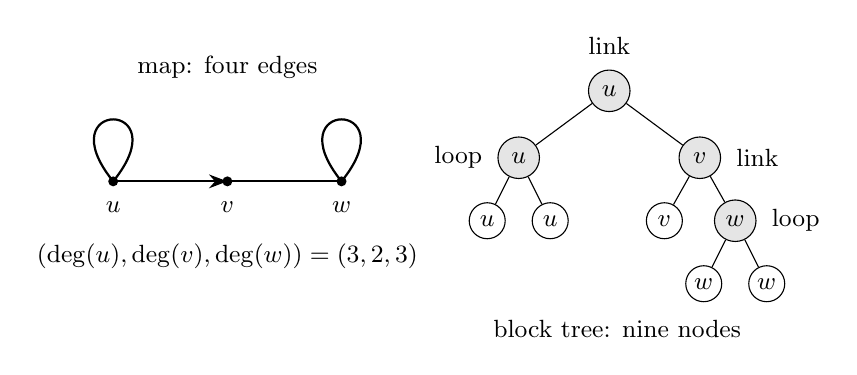
\begin{tikzpicture}[>=Stealth,font=\small]
 \begin{scope}[xshift=-3.5cm,yshift=0.4cm]
  \coordinate (u) at (0,0);
  \coordinate (v) at (1.45,0);
  \coordinate (w) at (2.9,0);
  \draw[thick,->] (u)--(v);
  \draw[thick] (v)--(w);
  \draw[thick] (u) .. controls (-0.85,1.05) and (0.85,1.05) .. (u);
  \draw[thick] (w) .. controls (2.05,1.05) and (3.75,1.05) .. (w);
  \foreach \x in {u,v,w}{\fill (\x) circle (1.8pt);}
  \node[below=4pt] at (u) {$u$};
  \node[below=4pt] at (v) {$v$};
  \node[below=4pt] at (w) {$w$};
  \node at (1.45,-0.95) {$(\deg(u),\deg(v),\deg(w))=(3,2,3)$};
  \node at (1.45,1.45) {map: four edges};
 \end{scope}
 \begin{scope}[xshift=2.8cm,yshift=1.55cm,
  block/.style={circle,draw,fill=black!10,inner sep=2pt,minimum size=15pt},
  leaf/.style={circle,draw,inner sep=1.5pt,minimum size=13pt}]
  \node[block] (r) at (0,0) {$u$};
  \node[block] (a) at (-1.15,-0.85) {$u$};
  \node[block] (b) at (1.15,-0.85) {$v$};
  \node[leaf] (a1) at (-1.55,-1.65) {$u$};
  \node[leaf] (a2) at (-0.75,-1.65) {$u$};
  \node[leaf] (b1) at (0.7,-1.65) {$v$};
  \node[block] (b2) at (1.6,-1.65) {$w$};
  \node[leaf] (c1) at (1.2,-2.45) {$w$};
  \node[leaf] (c2) at (2.0,-2.45) {$w$};
  \foreach \x/\y in {r/a,r/b,a/a1,a/a2,b/b1,b/b2,b2/c1,b2/c2}
   {\draw (\x)--(\y);}
  \node[above=2pt] at (r.north) {link};
  \node[left=2pt] at (a.west) {loop};
  \node[right=2pt] at (b.east) {link};
  \node[right=2pt] at (b2.east) {loop};
  \node at (0.1,-3.02) {block tree: nine nodes};
 \end{scope}
\end{tikzpicture}
\caption{Corner substitution and pole multiplicities. Shaded nodes carry
one-edge blocks; white nodes are trivial inserts. Node labels give
their poles in the map. The eight nonroot nodes have pole counts
$3,2,3$, exactly the vertex degrees. The arrow marks the root dart.}
\label{fig:corners}
\end{figure}


\section{Conditioned trees and uniform path sums}
\label{tree:section}

We isolate the probabilistic statement needed to pass from the block tree
to graph distances. Conditioned-tree height limits originate in
\cite{Aldous1993}; their stable-domain extension is developed in
\cite{Duquesne2003}. Joint depth-first process convergence to the same
excursion was proved by Marckert and Mokkadem under stronger moment
conditions~\cite{MarckertMokkadem2003}. We invoke the finite-variance,
attainable-size formulation of Broutin and
Marckert~\cite{BroutinMarckert2014} for the tree geometry.  We then prove a
uniform law of large numbers for marked ancestral paths, using only a
finite second offspring moment.

Let $\xi$ have distribution $(p_k)_{k\geq0}$ supported on the even
nonnegative integers, with
\begin{equation}
 p_0p_2>0,\qquad \E\xi=1,\qquad
 0<\sigma^2:=\operatorname{Var}(\xi)<\infty.
 \label{tree:assumptions}
\end{equation}
Write $\mathcal T$ for the corresponding plane Galton--Watson tree and
$\mathcal T_N$ for its law conditional on having $N$ nodes.  Its attainable
sizes are exactly the odd integers: every tree satisfies
$N-1=\sum_v\deg^+(v)$, and every odd size can be realized using only
offspring numbers zero and two.  All limits in this section run through
these odd integers.  Given the offspring numbers, attach independent
marks $A_v$ to the nodes, with a fixed law $\mathcal L_k$ at a node with
$k$ children.

Index the nodes in preorder by $v_0,\ldots,v_{N-1}$.  Let $H(v)$ denote
depth, put $H_j=H(v_j)$ for $j<N$ and $H_N=0$, and define the
exploration walk by
\begin{equation}
 W_0=0,\qquad W_{j+1}-W_j=\deg^+(v_j)-1
 \quad(0\leq j<N).
 \label{tree:walk-definition}
\end{equation}
Thus $W_j\geq0$ for $j<N$ and $W_N=-1$.  Interpolate both sequences
linearly between integer times, and write $W(v_j)=W_j$.

\begin{proposition}[Joint coding limit]
\label{tree:excursion}
Under \eqref{tree:assumptions},
\begin{equation}
 \left(\frac{W_{Nt}}{\sigma\sqrt N},
       \frac{\sigma H_{Nt}}{2\sqrt N}\right)_{0\leq t\leq1}
 \ \Longrightarrow\ (e(t),e(t))_{0\leq t\leq1}
 \quad\hbox{in }C([0,1],\R^2),
 \label{tree:walk-limit}
\end{equation}
where $e$ is a standard normalized Brownian excursion.
\end{proposition}
\begin{proof}
Broutin and Marckert's Theorem~3~\cite{BroutinMarckert2014} gives the
joint height and walk limit for uniform plane trees whose degree
frequencies and second moments converge to a critical finite-variance
law, with maximum degree $o(\sqrt N)$.  Their Lemma~11 verifies these
hypotheses in probability for conditioned critical Galton--Watson trees;
their Section~6 explicitly takes all attainable sizes.

Given the offspring counts $(n_k)$, our tree is uniform, since each
shape has probability $\prod_kp_k^{n_k}$.  To apply the deterministic
theorem to these random counts, take any subsequence and then a further
subsequence on which its degree hypotheses hold almost surely.
Conditional expectations of bounded continuous tests converge by the
theorem; dominated convergence removes the conditioning.  This proves
the limit along the full admissible sequence.

The source parametrizes height by $(N-1)t$.  Continuous-path tightness
makes the change to $Nt$ negligible before the last interval.  On that
interval, $H_{N-1}/\sqrt N\to0$ in probability because the limiting
excursion ends at zero, so appending $H_N=0$ is also harmless.  The marks
do not affect the tree-shape law.
\end{proof}

Put $\nu=\sigma^2/2$ and let $\Delta_N$ be the largest offspring number.

\begin{corollary}
\label{tree:maxdegree}
We have
\begin{equation}
 \max_v H(v)=O_{\P}(\sqrt N),\qquad
 \max_v W(v)=O_{\P}(\sqrt N),\qquad
 \Delta_N=o_{\P}(\sqrt N),
 \label{tree:degree-bound}
\end{equation}
and
\begin{equation}
 \max_v|W(v)-\nu H(v)|=o_{\P}(\sqrt N).
 \label{tree:walk-height-estimate}
\end{equation}
\end{corollary}
\begin{proof}
The height and walk bounds follow from Proposition~\ref{tree:excursion}.
Since both normalized processes converge jointly to the same excursion,
their uniform difference tends to zero in probability, proving
\eqref{tree:walk-height-estimate}.  Continuous-path tightness also makes
the largest walk increment divided by $\sqrt N$ tend to zero.  An
offspring number is a walk increment plus one.
\end{proof}

\begin{lemma}[Cost of conditioning]
\label{tree:conditioning}
As $N$ tends to infinity through odd integers,
\begin{equation}
 \pi_N:=\P(|\mathcal T|=N)
 \sim\frac{2}{\sigma\sqrt{2\pi}}N^{-3/2}.
 \label{tree:size-probability}
\end{equation}
\end{lemma}
\begin{proof}
Let $X_1,X_2,\ldots$ be independent with law $\xi-1$, and put
$S_r=\sum_{j=1}^rX_j$.  The exploration fills one waiting slot and
creates $\xi$ new ones at each step.  Thus total size $N$ means that
$S$ first reaches $-1$ at $N$.  A list of increments at least $-1$
totaling $-1$ has exactly one circular shift with this property: extend
the list periodically, decreasing its height by one per period, and
observe that its strict descending record endpoints occur once per
period.  Cyclic symmetry therefore gives the Otter--Dwass formula
(see also \cite[Theorem~15.5]{Janson2012})
\[
 \pi_N=\frac1N\P(S_N=-1).
\]
The lattice span of $X$ is exactly two because $-1$ and $1$ both have
positive probability.  At compatible sites $j\equiv r\pmod2$, the
finite-variance local limit estimate is
\[
 \P(S_r=j)=\frac{2}{\sigma\sqrt{2\pi r}}
             \exp\left(-\frac{j^2}{2r\sigma^2}\right)
             +o(r^{-1/2}),
\]
uniformly in $j$.  One can obtain this directly by Fourier inversion on
$[-\pi/2,\pi/2]$ with prefactor $1/\pi$: the characteristic function is
$1-\sigma^2\theta^2/2+o(\theta^2)$ near zero and has modulus strictly
less than one elsewhere on that interval.  Rescaling $\theta$ by
$r^{-1/2}$ gives the Gaussian integral, with uniformly vanishing
integrated error.  Taking $r=N$ and $j=-1$ proves the assertion.
\end{proof}

\subsection{A spine law and bounded labels}

For each strict ancestor of a node $v$, let $k$ be the ancestor's number
of children and $i\in\{1,\ldots,k\}$ the child leading toward $v$.
The waiting slots in the preorder exploration give
\begin{equation}
 W(v)=\sum_{\operatorname{path}(v)}(k-i),
 \qquad
 \widehat W(v):=\sum_{\operatorname{path}(v)}(i-1).
 \label{tree:waiting-slots}
\end{equation}
The second quantity is the preorder walk value at the corresponding
node after reversing every child order.  Reflection preserves the law
of $\mathcal T_N$ and preserves depths.  Hence
Corollary~\ref{tree:maxdegree} also gives
\begin{equation}
 \max_v|\widehat W(v)-\nu H(v)|=o_{\P}(\sqrt N).
 \label{tree:mirror-estimate}
\end{equation}
Only the tree shape is used here; no symmetry of the marks is required.

The size-biased spine construction is classical; see
Lyons, Pemantle, and Peres~\cite[Section~2]{LyonsPemantlePeres1995}.
For the marks and chosen child used here, define a probability law on
triples $(K,I,A)$ by
\begin{equation}
 \P_{\mathrm{sp}}(K=k,I=i,A\in B)=p_k\mathcal L_k(B),
 \qquad 1\leq i\leq k.
 \label{tree:spine-law}
\end{equation}
The total mass is $\E\xi=1$, and
\begin{equation}
 \E_{\mathrm{sp}}(K-I)=\frac{\E[\xi(\xi-1)]}{2}=\nu,
 \qquad \E_{\mathrm{sp}}K=2\nu+1<\infty.
 \label{tree:spine-means}
\end{equation}
For independent triples $Z_1,\ldots,Z_h$ with this law and every
nonnegative path function $F$, independence in the unconditioned tree
gives the path-counting identity
\begin{equation}
 \E\left[\sum_{H(v)=h}F(\operatorname{path}(v))\right]
 =\E_{\mathrm{sp}}F(Z_1,\ldots,Z_h).
 \label{tree:spine-identity}
\end{equation}
Indeed, at each ancestor one sums over its possible child choices; the
probability of each pair $(k,i)$, including its independent mark, is
exactly the factor in \eqref{tree:spine-law}.

For a label $b=b(k,i,A)$, set
\[
 B_b(v)=\sum_{\operatorname{path}(v)}b(k,i,A),\qquad
 \mu_b=\E_{\mathrm{sp}}b(K,I,A)
\]
whenever the expectation exists.

\begin{lemma}[Bounded path sums]
\label{tree:bounded-paths}
For every fixed bounded measurable real label $b$,
\begin{equation}
 \max_{v\in\mathcal T_N}|B_b(v)-\mu_bH(v)|
 =o_{\P}(\sqrt N).
 \label{tree:bounded-sums}
\end{equation}
\end{lemma}
\begin{proof}
Fix $C,\varepsilon>0$.  The exponential estimate for bounded independent
variables gives, uniformly for $h\leq C\sqrt N$,
\[
 \P_{\mathrm{sp}}\left(
 \left|\sum_{r=1}^h b(Z_r)-\mu_bh\right|>\varepsilon\sqrt N
 \right)\leq C' e^{-c'\sqrt N}.
\]
For short paths the event may be empty; otherwise the usual bound
$2\exp(-c\varepsilon^2N/h)$ gives the displayed estimate.  The
probability under $\mathcal T_N$ that any such path violates the desired
bound is at most
\[
 \pi_N^{-1}\sum_{h\leq C\sqrt N}C'e^{-c'\sqrt N}=o(1),
\]
by the unconditioned identity \eqref{tree:spine-identity} and
Lemma~\ref{tree:conditioning}.  Now let $C$ increase, using maximum-depth
tightness from Corollary~\ref{tree:maxdegree}.
\end{proof}

\subsection{Labels bounded by the offspring number}

We now allow labels that grow with the offspring number. The two
exploration orders control the sum of offspring numbers along every
ancestral path. Subtracting its bounded truncation will control the
remaining tail uniformly.

\begin{theorem}[Uniform marked path sums]
\label{tree:paths}
Let $b=b(k,i,A)$ be a fixed measurable label with $0\leq b\leq k$.
Then $\mu_b<\infty$ and
\begin{equation}
 \max_{v\in\mathcal T_N}|B_b(v)-\mu_bH(v)|=o_{\P}(\sqrt N),
 \qquad
 \max_{v\in\mathcal T_N}
 \left|B_b(v)-\frac{\mu_b}{\nu}W(v)\right|=o_{\P}(\sqrt N).
 \label{tree:marked-sums}
\end{equation}
\end{theorem}
\begin{proof}
The exact identities \eqref{tree:waiting-slots} give
\begin{equation}
 \sum_{\operatorname{path}(v)}k=W(v)+\widehat W(v)+H(v).
 \label{tree:total-label}
\end{equation}
By \eqref{tree:walk-height-estimate} and \eqref{tree:mirror-estimate},
this is $(2\nu+1)H(v)+o_{\P}(\sqrt N)$ uniformly in $v$.  For each
fixed $R$, Lemma~\ref{tree:bounded-paths} applies to the bounded label
$k\1_{\{k\leq R\}}$.  Subtracting its estimate yields
\begin{equation}
 \sum_{\operatorname{path}(v)}k\1_{\{k>R\}}
 =m_RH(v)+o_{\P}(\sqrt N)
 \quad\hbox{uniformly in }v,
 \qquad m_R:=\E_{\mathrm{sp}}[K\1_{\{K>R\}}].
 \label{tree:tail-estimate}
\end{equation}
The error statement here is for each fixed $R$.  Integrability of $K$
gives $m_R\to0$, and maximum-depth tightness consequently implies
\begin{equation}
 \lim_{R\to\infty}\limsup_{N\to\infty}
 \P\left(\max_v\sum_{\operatorname{path}(v)}
 k\1_{\{k>R\}}>\varepsilon\sqrt N\right)=0
 \quad(\varepsilon>0).
 \label{tree:uniform-tail}
\end{equation}
Apply Lemma~\ref{tree:bounded-paths} to $b\1_{\{k\leq R\}}$.
The discarded path sum is bounded by the tail in
\eqref{tree:uniform-tail}, and the discarded spine mean is bounded by
$m_R$.  Letting first $N$ and then $R$ tend to infinity proves the first
assertion.  The second follows from
\eqref{tree:walk-height-estimate} and $\nu>0$.
\end{proof}

This truncation uses $\E_{\mathrm{sp}}K=\E\xi^2<\infty$; it does not
require a second moment of the size-biased variable $K$, and hence does
not impose a third offspring moment.

We finish with a deterministic comparison for later use.

\begin{lemma}[Common ancestors and walk minima]
\label{tree:lca}
If $j\leq j'$ and $v_*$ is the lowest common ancestor of $v_j,v_{j'}$,
then
\begin{equation}
 W(v_*)\leq\min_{j\leq r\leq j'}W_r\leq W(v_*)+\Delta_N.
 \label{tree:lca-walk}
\end{equation}
\end{lemma}
\begin{proof}
Every intervening node is a descendant of $v_*$.  Its walk value is at
least $W(v_*)$ by \eqref{tree:waiting-slots}.  If $v_*=v_j$, the
upper bound is immediate.  Otherwise the interval contains the child of
$v_*$ leading toward $v_{j'}$; its walk value exceeds $W(v_*)$ by at
most the offspring number of $v_*$.
\end{proof}

\section{From the block tree to the map}\label{metric:section}

The mean block-distance comparison follows the general strategy for
subcritical graph classes~\cite[Section~5]{PanagiotouStuflerWeller2016}
and tree-like maps~\cite[preprint Section~6.8]{Stufler2020}.
Here Theorem~\ref{tree:paths} supplies the required uniformity under
only finite offspring variance. We also retain the exact corner-mass
calculation, as in~\cite[Section~9]{Stufler2026}, because the conclusion
specifies the degree probability measure.

Let $\mathsf T_N$ be the conditioned marked tree of
Proposition~\ref{block:finite-law}, where $N=2n+1$. Its map has the
required marginal law of $M_n$. Write $\pi(w)$ for the pole of a tree
node $w$. For a strict ancestor with $k$ children, block mark $B$, and
selected child $i$, put
\[
 g(k,i,B)=d_B\big(\text{pole of }B,\text{vertex of corner }i\big),
 \qquad \beta=\E_{\rm sp}g.
\]
The expectation is under the spine law \eqref{tree:spine-law}, and
$d_B$ uses all block edges. Since a block has $k/2$ edges,
$0\le g\le k$. Therefore
\begin{equation}\label{metric:beta}
 0<\beta<\infty.
\end{equation}
Finiteness follows from $\E_{\rm sp}k=\E\xi^2<\infty$.
For positivity, a one-link block and its corner at the endpoint
opposite the pole have positive spine probability, and their distance
is one.

Let $G(w)$ be the sum of these $g$ labels over the strict ancestors of
$w$. By Theorem~\ref{tree:paths} and the coding estimates in
Section~\ref{tree:section}, with $\nu=\sigma^2/2$,
\begin{equation}\label{metric:uniform-poles}
 \max_{w\in\mathsf T_N}
 \left|G(w)-\beta H(w)\right|=\op(\sqrt N),\qquad
 \max_{w\in\mathsf T_N}
 \left|G(w)-\frac{\beta}{\nu}W(w)\right|=\op(\sqrt N).
\end{equation}

\subsection{Uniform comparison of distances}

\begin{lemma}[Distances between poles]\label{metric:poles}
Let $w_*$ be the last common ancestor of two tree nodes $w,w'$.
If $\Delta$ is the maximum offspring number, then
\[
 \left|d_{M_n}\big(\pi(w),\pi(w')\big)
       -\big(G(w)+G(w')-2G(w_*)\big)\right|\le2\Delta.
\]
The map $\pi$ from tree nodes to map vertices is onto.
\end{lemma}

\begin{proof}
Every inserted map meets the preceding part at its pole only.
An excursion from a block into an attached submap must return to the
same vertex, so attachments cannot shorten distances within a block.
Moving from an ancestor pole to a descendant pole therefore adds
the distances $g$ along their chain of blocks.

If one of $w,w'$ is their last common ancestor, this proves the
displayed comparison with zero error. Otherwise let $x,x'$ be the two
selected corner vertices in the block of $w_*$. The route through
the pole of that block has length
$d_B(x,\pi(w_*))+d_B(\pi(w_*),x')$ within the block, whereas the
shortest route uses $d_B(x,x')$. Their difference lies between zero
and twice the diameter of $B$, and that diameter is at most its
number of edges, hence at most $\Delta$. Outside the common block
the distances add exactly as above. The same argument allows
coincident poles and loop blocks.

Every vertex of the nonempty map is incident to at least one edge,
and hence to a corner in one of its blocks. That corner is a child
slot, whose child's pole is the given vertex. Thus every map vertex
is the pole of a nonroot node.
\end{proof}

Index the nodes by $j=0,\ldots,N-1$ in preorder. Combining
Lemma~\ref{metric:poles}, \eqref{metric:uniform-poles}, and
Lemma~\ref{tree:lca}, and using $\Delta=\op(\sqrt N)$, gives
\begin{equation}\label{metric:walk-comparison}
 \max_{0\le j\le j'<N}
 \left|d_{M_n}\big(\pi(j),\pi(j')\big)
  -\frac{\beta}{\nu}
       \left(W_j+W_{j'}-2\min_{j\le r\le j'}W_r\right)\right|
   =\op(\sqrt N).
\end{equation}
In particular, the comparison is uniform over every map vertex,
including vertices in the largest blocks.

\subsection{The degree measure}

\begin{lemma}[Corner mass]\label{metric:measure}
The uniform probability measure on the $N-1=2n$ nonroot tree nodes,
pushed forward by $\pi$, is exactly $\mu_n$.
\end{lemma}

\begin{proof}
Each nonroot node occupies one corner of its parent block, and every
block corner is occupied once, including the corners whose inserts
are trivial leaves. At a map vertex $v$, summing these corner counts
over the blocks gives $\deg_{M_n}(v)$: each incident dart belongs to
one block, and each block has one corner per incident dart. A loop
contributes two darts and two corners at its vertex.
Division by the total $2n$ proves the assertion.
\end{proof}

If $\bar\mu_n$ is instead the pushforward of uniform probability on
all $N$ nodes, then
\begin{equation}\label{metric:mass-error}
 \bar\mu_n=\frac{N-1}{N}\mu_n+\frac1N\delta_{\pi(0)},
 \qquad
 \|\bar\mu_n-\mu_n\|_{\rm TV}\le\frac1N.
\end{equation}
The measure identity is thus independent of the sizes and shapes of
the individual blocks.

\subsection{A correspondence estimate}

For completeness we state the elementary estimate used to pass to
metric probability spaces. A \emph{correspondence} between $X$ and
$Y$ is a relation $\mathcal R\subseteq X\times Y$ projecting onto both
spaces. Its distortion is
\[
 \operatorname{dis}(\mathcal R)
 =\sup_{\substack{(x,y),(x',y')\in\mathcal R}}
       |d_X(x,x')-d_Y(y,y')|.
\]
The Gromov--Hausdorff--Prokhorov distance is the infimum, over common
isometric embeddings, of the maximum of the Hausdorff distance
between the embedded spaces and the Prokhorov distance between their
probability measures.

\begin{lemma}[Metric and mass comparison]\label{metric:ghp}
Suppose a correspondence between compact metric probability spaces
has distortion at most $\varepsilon>0$, and a coupling of their
probability measures is supported on the correspondence. Their
Gromov--Hausdorff--Prokhorov distance is at most $\varepsilon$.
If one marginal of that coupling differs from the desired measure
by total variation at most $\eta$, the bound is
$\varepsilon+\eta$.
\end{lemma}

\begin{proof}
Join corresponding points by links of length $\varepsilon$, and
use the induced shortest-chain distance on the disjoint union.
This preserves the distances within each original space.
Indeed, a segment leaving one space and returning to it can be
replaced by a segment inside that space: the two linking lengths
are $2\varepsilon$, whereas the difference of the distances between
the corresponding endpoints is at most $\varepsilon$.
Every point is within $\varepsilon$ of the other space, giving the
Hausdorff bound. The coupling places every pair at distance at most
$\varepsilon$, which gives the Prokhorov bound directly from its
defining neighborhood inequalities. Changing one marginal by
total variation $\eta$ increases these inequalities, and hence the
Prokhorov bound, by at most $\eta$.
\end{proof}

For a nonnegative continuous function $f$ on $[0,1]$ with
$f(0)=f(1)=0$, define $d_f$ by the same formula as $d_e$, and denote
its quotient metric probability space by $\mathcal T_f$.
The interval-minimum formula gives the triangle inequality for $d_f$.
The quotient projection is continuous, since
$d_f(s,t)$ is at most twice the oscillation of $f$ on the interval
between $s$ and $t$. Thus $\mathcal T_f$ is compact.
Relating equal-time representatives in $\mathcal T_f$ and
$\mathcal T_{\tilde f}$ gives a correspondence of distortion at most
$4\|f-\tilde f\|_\infty$ and a coupling from one uniform time.
Lemma~\ref{metric:ghp} therefore proves continuity of
\[
 f\longmapsto \mathcal T_f
\]
from the uniform norm to the Gromov--Hausdorff--Prokhorov topology.

\subsection{Proof of the main theorem}

\begin{proof}[Proof of Theorem~\ref{thm:main}]
Define
\begin{equation}\label{metric:constant}
 c(q)=\frac{\nu}{\sqrt2\,\beta\sigma}
     =\frac{\sigma}{2\sqrt2\,\beta}.
\end{equation}
Equations~\eqref{block:moments} and \eqref{metric:beta} show that this
constant is deterministic, positive, and finite for every fixed $q>4$.

Let $f_N$ interpolate $W_j/(\sigma\sqrt N)$ at $j/N$ for
$0\le j<N$, and set $f_N(1)=0$. It is nonnegative and has zero
endpoints. Replacing the exploration walk's last value
$W_N=-1$ by zero changes its normalized interpolation by at most
$1/(\sigma\sqrt N)$. Proposition~\ref{tree:excursion} consequently gives
\[
 f_N\Longrightarrow e
 \qquad\text{in }C([0,1]).
\]
For grid points $j/N,j'/N$, the comparison
\eqref{metric:walk-comparison} and the identity $N=2n+1$ imply
\[
 \max_{j,j'<N}
 \left|
  \frac{c(q)}{\sqrt n}\,
     d_{M_n}\big(\pi(j),\pi(j')\big)
  -\sqrt{\frac{N}{2n}}\,
     d_{f_N}(j/N,j'/N)
 \right|=\op(1).
\]
Since $\sqrt{N/(2n)}\to1$ and $\|f_N\|_\infty$ is tight, that
deterministic factor may be replaced by one.

For $s\in[0,1]$, put $j_N(s)=\min\{\lfloor Ns\rfloor,N-1\}$ and
write $[s]$ for its class in $\mathcal T_{f_N}$. The relation
\[
 \mathcal R_N=\{(\pi(j_N(s)),[s]):s\in[0,1]\}
\]
is a correspondence by Lemma~\ref{metric:poles}.
Rounding times changes a $d_{f_N}$ distance by at most
$4\omega_{f_N}(1/N)$, where $\omega$ is the uniform modulus of
continuity. Continuous-path tightness makes this error tend to zero
in probability. The correspondence therefore has distortion
$\op(1)$ for the rescaled map metric.

A Lebesgue-uniform time couples the probability measure of
$\mathcal T_{f_N}$ to $\bar\mu_n$ exactly, since each of the $N$
preorder cells has length $1/N$. By
Lemma~\ref{metric:ghp} and \eqref{metric:mass-error}, the
Gromov--Hausdorff--Prokhorov distance from the rescaled map with
measure $\mu_n$ to $\mathcal T_{f_N}$ tends to zero in probability.
The continuity established above and $f_N\Longrightarrow e$ prove
the claimed convergence to $(\mathcal T_e,d_e,\mu_e)$.

Proposition~\ref{block:finite-law} applies to every $n\ge1$, and
the conditioned-tree results hold through all the corresponding
odd sizes. The proof uses only the map marginal and all-edge
block distances, so its conclusion is precisely the unrooted,
undecorated metric probability limit stated in the theorem.
\end{proof}

\begin{thebibliography}{99}

\bibitem{AddarioBerry2019}L.~Addario-Berry,
\emph{A probabilistic approach to block sizes in random maps},
ALEA Lat. Am. J. Probab. Math. Stat. \textbf{16} (2019), 1--13.
\href{https://doi.org/10.30757/ALEA.v16-01}{doi:10.30757/ALEA.v16-01}.

\bibitem{Aldous1993}D.~Aldous,
\emph{The continuum random tree III},
Ann. Probab. \textbf{21} (1993), no.~1, 248--289.
\href{https://doi.org/10.1214/aop/1176989404}{doi:10.1214/aop/1176989404}.

\bibitem{Bernardi2007}O.~Bernardi,
\emph{Bijective counting of tree-rooted maps and shuffles of parenthesis systems},
Electron. J. Combin. \textbf{14} (2007), R9.
\href{https://doi.org/10.37236/928}{doi:10.37236/928}.

\bibitem{Bernardi2008}O.~Bernardi,
\emph{A characterization of the Tutte polynomial via combinatorial embeddings},
Ann. Comb. \textbf{12} (2008), no.~2, 139--153.
\href{https://doi.org/10.1007/s00026-008-0343-4}{doi:10.1007/s00026-008-0343-4}.

\bibitem{Bernardi2008Subgraphs}O.~Bernardi,
\emph{Tutte polynomial, subgraphs, orientations and sandpile model: new connections via embeddings},
Electronic Journal of Combinatorics \textbf{15} (2008), no.~1, R109.
\href{https://doi.org/10.37236/833}{doi:10.37236/833}.

\bibitem{BroutinMarckert2014}N.~Broutin and J.-F.~Marckert,
\emph{Asymptotics of trees with a prescribed degree sequence and applications},
Random Structures Algorithms \textbf{44} (2014), no.~3, 290--316.
\href{https://doi.org/10.1002/rsa.20463}{doi:10.1002/rsa.20463}.
Preprint: \href{https://arxiv.org/abs/1110.5203v3}{arXiv:1110.5203v3}.

\bibitem{Duquesne2003}T.~Duquesne,
\emph{A limit theorem for the contour process of conditioned Galton--Watson trees},
Ann. Probab. \textbf{31} (2003), no.~2, 996--1027.
\href{https://doi.org/10.1214/aop/1048516543}{doi:10.1214/aop/1048516543}.

\bibitem{Feng2026}Y.~Feng,
\emph{Triviality of critical Fortuin--Kasteleyn decorated planar maps for $q>4$},
Probab. Theory Related Fields \textbf{194} (2026), 299--331.
\href{https://doi.org/10.1007/s00440-025-01424-2}{doi:10.1007/s00440-025-01424-2}.

\bibitem{FortuinKasteleyn1972}C.~M.~Fortuin and P.~W.~Kasteleyn,
\emph{On the random-cluster model. I. Introduction and relation to other models},
Physica \textbf{57} (1972), no.~4, 536--564.
\href{https://doi.org/10.1016/0031-8914(72)90045-6}{doi:10.1016/0031-8914(72)90045-6}.

\bibitem{Janson2012}S.~Janson,
\emph{Simply generated trees, conditioned Galton--Watson trees, random allocations and condensation},
Probability Surveys \textbf{9} (2012), 103--252.
\href{https://doi.org/10.1214/11-PS188}{doi:10.1214/11-PS188}.

\bibitem{LyonsPemantlePeres1995}R.~Lyons, R.~Pemantle, and Y.~Peres,
\emph{Conceptual proofs of $L\log L$ criteria for mean behavior of branching processes},
Annals of Probability \textbf{23} (1995), no.~3, 1125--1138.
\href{https://arxiv.org/abs/math/0404083}{arXiv:math/0404083}.

\bibitem{MarckertMokkadem2003}J.-F.~Marckert and A.~Mokkadem,
\emph{The depth first processes of Galton--Watson trees converge to the same Brownian excursion},
Annals of Probability \textbf{31} (2003), no.~3, 1655--1678.

\bibitem{Mullin1967}R.~C.~Mullin,
\emph{On the enumeration of tree-rooted maps},
Canad. J. Math. \textbf{19} (1967), 174--183.
\href{https://doi.org/10.4153/CJM-1967-010-x}{doi:10.4153/CJM-1967-010-x}.

\bibitem{SubcriticalConformal2026}OpenAI,
\emph{Canonical conformal limits of subcritical FK planar maps},
OpenAI Math Release preprint
\href{https://github.com/openai/math/blob/main/preprints/Canonical-conformal-limits-of-subcritical-FK-planar-maps-September-24-2026/main.pdf}{OAI:Canonical-conformal-limits-of-subcritical-FK-planar-maps-September-24-2026},
2026.

\bibitem{SubcriticalMetric2026}OpenAI,
\emph{Metric-measure limits of subcritical FK and spanning-tree planar maps},
OpenAI Math Release preprint
\href{https://github.com/openai/math/blob/main/preprints/Metric-measure-limits-of-subcritical-FK-and-spanning-tree-planar-maps-September-24-2026/main.pdf}{OAI:Metric-measure-limits-of-subcritical-FK-and-spanning-tree-planar-maps-September-24-2026},
2026.

\bibitem{CriticalFK2026}OpenAI,
\emph{The critical Liouville quantum sphere and geometric limits of FK maps at $q=4$},
OpenAI Math Release preprint
\href{https://github.com/openai/math/blob/main/preprints/The-critical-Liouville-quantum-sphere-and-geometric-limits-of-FK-maps-at-q-equals-4-September-24-2026/main.pdf}{OAI:The-critical-Liouville-quantum-sphere-and-geometric-limits-of-FK-maps-at-q-equals-4-September-24-2026},
2026.

\bibitem{PanagiotouStuflerWeller2016}K.~Panagiotou, B.~Stufler, and K.~Weller,
\emph{Scaling limits of random graphs from subcritical classes},
Annals of Probability \textbf{44} (2016), no.~5, 3291--3334.
\href{https://doi.org/10.1214/15-AOP1048}{doi:10.1214/15-AOP1048}.

\bibitem{Sheffield2016}S.~Sheffield,
\emph{Quantum gravity and inventory accumulation},
Ann. Probab. \textbf{44} (2016), no.~6, 3804--3848.
\href{https://doi.org/10.1214/15-AOP1061}{doi:10.1214/15-AOP1061}.

\bibitem{Stufler2020}B.~Stufler,
\emph{Limits of random tree-like discrete structures},
Probability Surveys \textbf{17} (2020), 318--477.
\href{https://doi.org/10.1214/19-PS338}{doi:10.1214/19-PS338}.
Preprint: \href{https://arxiv.org/abs/1612.02580v2}{arXiv:1612.02580v2}.

\bibitem{Stufler2026}B.~Stufler,
\emph{Non-bijective scaling limits and phase transitions of planar maps},
\href{https://arxiv.org/abs/2608.21063v1}{arXiv:2608.21063v1} (2026).

\bibitem{Tutte1963}W.~T.~Tutte,
\emph{A census of planar maps},
Canad. J. Math. \textbf{15} (1963), 249--271.
\href{https://doi.org/10.4153/CJM-1963-029-x}{doi:10.4153/CJM-1963-029-x}.

\end{thebibliography}


\end{document}
